\documentclass[a4paper,11pt]{article}

\usepackage[utf8]{inputenc}
\usepackage[swedish]{babel}
\usepackage[top=1in,bottom=1in,left=1in,right=1in,headsep=.5in]{geometry}
\usepackage{hyperref}
\usepackage{graphicx}
\usepackage{pdfpages}

\usepackage{tikz}
\usetikzlibrary{shapes.geometric, shapes.misc, arrows, calc}

\usepackage{array}
\newcolumntype{L}[1]{>{\raggedright\let\newline\\\arraybackslash\hspace{0pt}}m{#1}}
\newcolumntype{C}[1]{>{\centering\let\newline\\\arraybackslash\hspace{0pt}}m{#1}}
\newcolumntype{R}[1]{>{\raggedleft\let\newline\\\arraybackslash\hspace{0pt}}m{#1}}

\usepackage[yyyymmdd,hhmmss]{datetime}
\renewcommand{\dateseparator}{-}

\usepackage{mathptmx}    %Times Roman font
\usepackage{helvet}    %Helvetica, served as a model for arial
\usepackage{anyfontsize}

\usepackage[tocgraduated]{tocstyle}
\usetocstyle{allwithdot}

\usepackage[titletoc,title]{appendix}

\usepackage[backend=bibtex,style=authoryear,maxcitenames=2,maxbibnames=9]{biblatex} %Harvard-style citations
\setlength{\bibitemsep}{\baselineskip}	%vertical space between bibliography items

\usepackage{fancyhdr}
\fancypagestyle{intro}{
    \fancyhf{}
    \fancyhead[C]{\LIPSprojekttitel}
    \fancyhead[R]{\today} 
    \fancyfoot[L]{\LIPSkursnamn \\ \LIPSdokumenttyp}
    \fancyfoot[C]{\phantom{text}\roman{page}}
    \fancyfoot[R]{\LIPSprojektgrupp \\ \LIPSgruppepost} 
    \renewcommand{\headrulewidth}{0.4pt}
    \renewcommand{\footrulewidth}{0.4pt}}
\fancypagestyle{content}{
    \fancyhf{}
    \fancyhead[C]{\LIPSprojekttitel}
    \fancyhead[R]{\today} 
    \fancyfoot[L]{\LIPSkursnamn \\ \LIPSdokumenttyp}
    \fancyfoot[C]{\phantom{text}\thepage}
    \fancyfoot[R]{\LIPSprojektgrupp \\ \LIPSgruppepost} 
    \renewcommand{\headrulewidth}{0.4pt}
    \renewcommand{\footrulewidth}{0.4pt}}

\usepackage{titlesec}
\titleformat{\section}
    {\normalfont\sffamily\Large\bfseries}
    {\thesection}{1em}{}
\titleformat{\subsection}
    {\normalfont\sffamily\large\bfseries}
    {\thesubsection}{1em}{}
\titleformat{\subsubsection}
    {\normalfont\sffamily\bfseries}
    {\thesubsubsection}{1em}{}

\newcommand{\LIPSartaltermin}{2016/HT}
\newcommand{\LIPSkursnamn}{TSEA29}
\newcommand{\LIPSprojekttitel}{Kartrobot}
\newcommand{\LIPSprojektgrupp}{Grupp 1}
\newcommand{\LIPSgruppepost}{\href{mailto:kmm_2016_grupp1@liuonline.onmicrosoft.com}{{\small kmm\_2016\_grupp1@liuonline.onmicrosoft.com}}}
\newcommand{\LIPSgrupphemsida}{}
\newcommand{\LIPSkund}{ISY, Linköpings universitet, 581\,83 Linköping}
\newcommand{\LIPSkundkontakt}{Mattias Krysander, 013-282198, matkr@isy.liu.se}
\newcommand{\LIPSkursansvarig}{Tomas Svensson, 013-281368, Tomas.Svensson@liu.se}
\newcommand{\LIPShandledare}{Olov Andersson, 013-282658, olov@isy.liu.se}
\newcommand{\LIPSdokumenttyp}{Designspecifikation}
\newcommand{\LIPSredaktor}{Jag måste skriva något här annars kan jag inte kompilera dokumentet}    %TODO Välj redaktör. Borde vara HV eller MV enligt projektplan

\newcommand{\LIPSversion}{0.1}
\newcommand{\LIPSgranskare}{}
\newcommand{\LIPSgranskatdatum}{}
\newcommand{\LIPSgodkannare}{}
\newcommand{\LIPSgodkantdatum}{}

\addbibresource{bibliography.bib}
\newcommand{\LIPStitelsida}{
\vspace*{200pt}
\renewcommand{\familydefault}{\sfdefault}	%Sans-serif
\normalfont
\begin{center}
{\fontsize{18}{22}\selectfont \textbf{\MakeUppercase{\LIPSdokumenttyp}}}
\end{center}
\begin{center}
{\fontsize{12}{14}\selectfont \LIPSredaktor \\[8pt] Version \LIPSversion}
\end{center}
\vspace*{220pt}
\begin{center}
{\fontsize{12}{14}\selectfont Status}
\end{center}
\begin{center}
\setlength\extrarowheight{2pt}
\begin{tabular}{| L{100pt} | L{100pt} | L{100pt} |}
\hline 
Granskad & \LIPSgranskare & \LIPSgranskatdatum \\
\hline 
Godkänd & \LIPSgodkannare & \LIPSgodkantdatum \\ 
\hline 
\end{tabular} 
\end{center}
\renewcommand{\familydefault}{\rmdefault}	%Back to serifs
\normalfont
}


\newenvironment{LIPSprojektidentitet}{%
\vspace*{200pt}
\renewcommand{\familydefault}{\sfdefault}	%Sans-serif
\normalfont
\begin{center}
{\fontsize{16}{19}\selectfont \textbf{PROJEKTIDENTITET}}
\end{center}
\renewcommand{\familydefault}{\rmdefault}	%Back to serifs
\normalfont
\begin{center}
\LIPSartaltermin, \LIPSprojektgrupp \\ Linköpings tekniska högskola, ISY
\end{center}
\renewcommand{\familydefault}{\sfdefault}	%Sans-serif
\normalfont
\vspace*{10pt}
\begin{center}
\setlength\extrarowheight{2pt}
\begin{tabular}{| L{100pt} | L{150pt} | L{150pt} |}
\hline
\textbf{Namn} & \textbf{Ansvar} & \textbf{E-post} \\
}%
{%
\hline
\end{tabular} 
\end{center}
\renewcommand{\familydefault}{\rmdefault}	%Back to serifs
\normalfont
\begin{center}
\textbf{E-postlista för hela gruppen:} \LIPSgruppepost \\
\textbf{Hemsida:} \LIPSgrupphemsida \\
\vspace*{15pt}
\textbf{Kund:} \LIPSkund \\
\textbf{Kontaktperson hos kund:} \LIPSkundkontakt \\
\vspace*{15pt}
\textbf{Kursansvarig:} \LIPSkursansvarig \\
\textbf{Handledare:} \LIPShandledare \\
\end{center}
}
\newcommand{\LIPSgruppmedlem}[3]{\hline {#1} & {#2} & \href{mailto:{#3}}{{#3}} \\}

\newenvironment{LIPSdokumenthistorik}{%
\vspace*{100pt}
\renewcommand{\familydefault}{\sfdefault}	%Sans-serif
\normalfont
\begin{center}
{\fontsize{14}{17}\selectfont \textbf{Dokumenthistorik}}
\end{center}
\begin{center}
\setlength\extrarowheight{2pt}
\begin{tabular}{| L{50pt} | L{60pt} | L{150pt} | L{60pt} | L{55pt} |}
\hline
\textbf{Version} & \textbf{Datum} & \textbf{Utförda förändringar} & \textbf{Utförda av} & \textbf{Granskad} \\
}%
{%
\hline
\end{tabular} 
\end{center}
\renewcommand{\familydefault}{\rmdefault}	%Back to serifs
\normalfont
}
\newcommand{\LIPSversionsinfo}[5]{\hline {#1} & {#2} & {#3} & {#4} & {#5} \\}

\newcounter{LIPSkravnummer}
\newcounter{LIPSunderkravnummer}[LIPSkravnummer]
\newenvironment{LIPSkravlista}{%
\renewcommand{\familydefault}{\sfdefault}	%Sans-serif
\normalfont
 \setlength\extrarowheight{2pt}
  \begin{tabular}{| L{30pt } | L{60pt} | L{250pt} | L{50pt} |}
    }%
  {%
    \hline
  \end{tabular}
\renewcommand{\familydefault}{\rmdefault}	%Back to serifs
\normalfont
}
\newcommand{\LIPSkrav}[3]{\hline\stepcounter{LIPSkravnummer}\textbf{\arabic{LIPSkravnummer}} & \textbf{{#1}} & {#2} & \textbf{{#3}} \\}

\newcommand{\LIPSkravDemo}[3]{\hline\textbf{X} & \textbf{{#1}} & {#2} & \textbf{{#3}} \\}

\newcommand{\LIPSunderkrav}[3]{\hline\stepcounter{LIPSunderkravnummer}\textbf{\arabic{LIPSkravnummer}\Alph{LIPSunderkravnummer}} & \textbf{{#1}} & {#2} & \textbf{{#3}} \\}


\newenvironment{LIPSleveranslista}{
\renewcommand{\familydefault}{\sfdefault}	%Sans-serif
\normalfont
	\setlength\extrarowheight{2pt}
	\begin{tabular}{| L{25mm} | L{25mm} | L{55mm} | L{25mm} | L{5mm} |} 
	}
	{
		\hline
	\end{tabular}
\renewcommand{\familydefault}{\rmdefault}	%Back to serifs
\normalfont
}
\newcommand{\LIPSleverans}[4]{ \hline\stepcounter{LIPSkravnummer}\textbf{Krav nr \arabic{LIPSkravnummer}}&\textbf{{#1}}&{#2}&\textbf{{#3}}&\textbf{{#4}}\\}


\newenvironment{LIPSdokumentlista}{%
	\renewcommand{\familydefault}{\sfdefault}	%Sans-serif
	\normalfont
	\setlength\extrarowheight{2pt}
	\begin{tabular}{| L{40mm} | L{13mm} | L{50mm} | L{19mm} | L{14mm} |} 
		
		\hline
		\textbf{Dokument} & \textbf{Språk} & \textbf{Syfte/Innehåll} & \textbf{Målgrupp} & \textbf{Format} \\
	}%
	{%
		\hline
	\end{tabular}
	\renewcommand{\familydefault}{\rmdefault}	%Back to serifs
	\normalfont
}
\newcommand{\LIPSdokument}[5]{\hline {#1} & {#2} & {#3} & {#4} & {#5}\\}


\begin{document}

\pagestyle{intro}
\LIPStitelsida
\clearpage
\begin{LIPSprojektidentitet}
    \LIPSgruppmedlem{Hannes Haglund}{Designansvarig mjukvara (MV)}{hanha265@student.liu.se}
    \LIPSgruppmedlem{Felix Härnström}{Projektledare (PL)}{felha423@student.liu.se}
    \LIPSgruppmedlem{Jani Jokinen}{Leveransansvarig (LEV)}{janjo273@student.liu.se}
    \LIPSgruppmedlem{Silas Lenz}{Testansvarig (TST)}{sille914@student.liu.se}
    \LIPSgruppmedlem{Daniel Månsson}{Designansvarig hårdvara (HV)}{danma344@student.liu.se}
    \LIPSgruppmedlem{Emil Norberg}{Dokumentansvarig (DOK)}{emino969@student.liu.se}
\end{LIPSprojektidentitet}

\clearpage
\renewcommand{\familydefault}{\sfdefault}	%Sans-serif
\normalfont
\tableofcontents
\renewcommand{\familydefault}{\rmdefault}	%Back to serifs
\normalfont
\clearpage
\begin{LIPSdokumenthistorik}
    \LIPSversionsinfo{0.1}{2016-09-22}{Första utkastet}{}{}
\end{LIPSdokumenthistorik}
\clearpage
\setcounter{page}{1}
\pagestyle{content}

\section{Systemöversikt}
I detta projekt konstrueras en robot med förmågan att kartlägga rum som specificeras enligt \cite{coursespec}. Detta gör den genom att förflytta sig i rummet (med manuell eller autonom styrning) och skanna med en avståndskänslig laser. Kommandon och resultat skickas till respektive från en extern PC via ett blåtandsgränssnitt. Se figur \ref{fig:overview} för en bild på roboten i sin omgivning.

\begin{figure}[h!]
    \makebox[\textwidth][c]{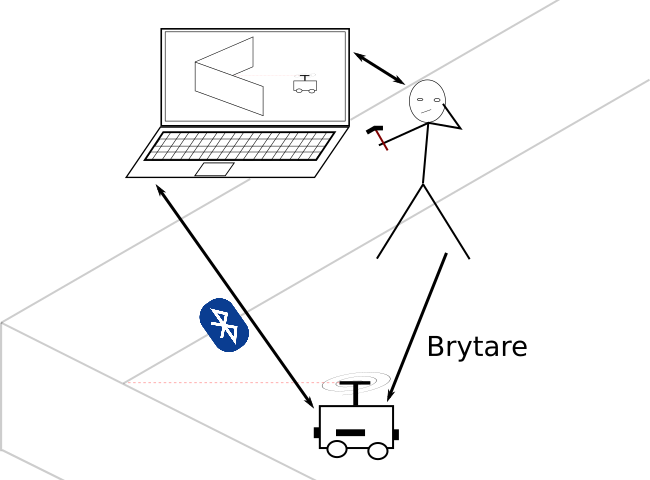
\includegraphics[width=1\textwidth]{overview.png}}
    \caption{Systemet i dess omgivning.}
    \label{fig:overview}
\end{figure}

\noindent
Systemet innehåller fyra kommunicerande datorer (enheter) med egna ansvarsområden och uppgifter:

\begin{itemize}
\item Sensorenhet (se kapitel \ref{sec:system1})
\item Styrenhet (se kapitel \ref{sec:system2})
\item Kommunikations- och kontrollenhet (se kapitel \ref{sec:system3})
\item Extern PC (se kapitel \ref{sec:system4})
\end{itemize}

\noindent
Sensorenheten behandlar data från systemets olika sensorer, för att sedan skicka vidare datan på ett mer användbart format med minimala läsfel.

Styrenheten ansvarar för att omvandla högnivåkommandon till lågnivåkommandon och propagera dessa till systemets olika motorer och servos.

Kommunikations- och kontrollenheten är den centrala hjärnan i systemet, som skickar kommandon till de andra enheterna. I det manuella läget utför den kommandon som kommer från den externa PC:n, och i det autonoma bestämmer den själv bästa tillvägagångssätt för att systemet ska kunna kartlägga rummet.

På den externa PC:n finner vi ett användargränssnitt där en människa kan läsa av resultat, avlusningsdata, samt skicka kommandon till roboten om denna befinner sig i det manuella läget.

I figur \ref{fig:modules} beskrivs det grafiskt hur dessa moduler kommunicerar med varandra. Mer detaljerade blockschema finns till varje modul, samt en fullständig översikt i figur \ref{fig:modulesDetailed}.

\begin{figure}
    \makebox[\textwidth][c]{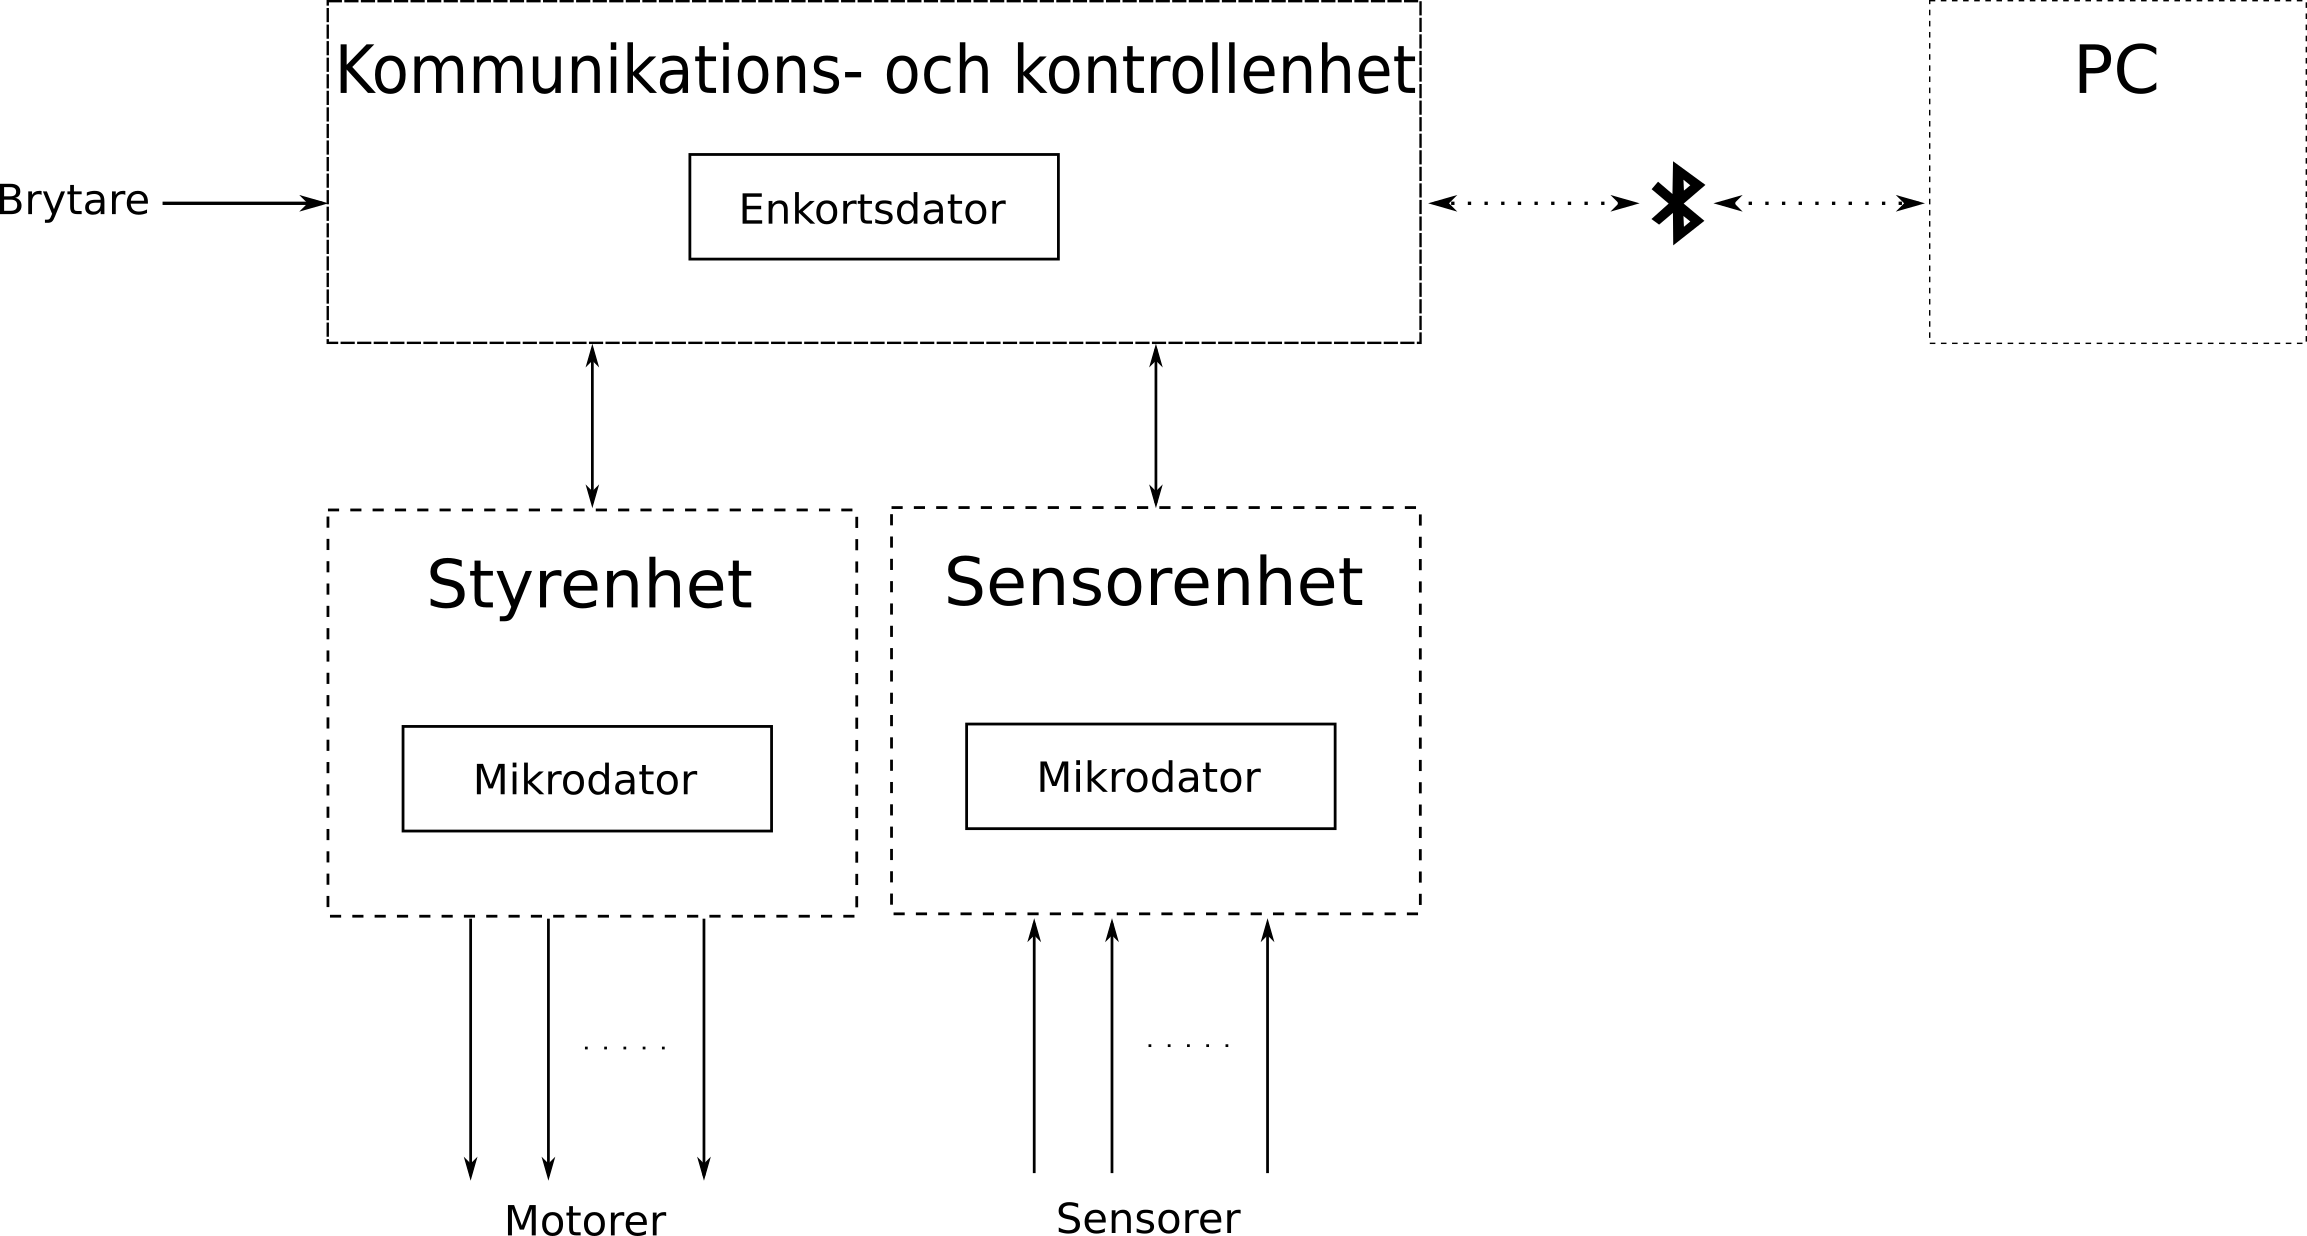
\includegraphics[width=1\textwidth]{modules.png}}
    \caption{Modulöversikt.}
    \label{fig:modules}
\end{figure}

\noindent
Robotens hårdvara är monterad ovanpå dess chassi, en modell som går under namnet \cite{terminator}. Denna kommer med fyra hjul påmonterade, som används för att roboten ska kunna ta sig runt i rummet. Ytterliggare ett servo, monteras på toppen av roboten.

Ovanpå denna sitter den avståndskänsliga lasern LIDAR - systemets främsta vapen vad gäller rumskanning. Ytterligare sensorer hittas på tre av robotens fyra sidor: IR-sensorer för bättre kontroll under körning. Ingen monteras längst fram på chassit, eftersom LIDARn täcker den funktionaliteten då roboten rör på sig.

Vidare monteras ett gyro (modell MLX90609) i mitten av roboten för att den ska kunna rotera mer precist.

I bilaga \ref{app:placement} hittar ni en grafisk beskrivning av hårdvarans placering.

\subsection{Kommunikation}
För kommunikation mellan Kommunikation- och kontrollenheten (se kapitel \ref{sec:system3}) och sensorenheten samt styrenheten (se kapitel \ref{sec:system2} respektive \ref{sec:system3}) används UART-bussar. Då Raspberry pi:n som används i kontrollenheten saknar inbyggd UART så används USB-till-UART-moduler. Vidare så kommunicerar Kommunikation- och kontrollenheten via blåtand med PC-mjukvaran (se kapitel \ref{sec:system4}).

Vidare är en UART-buss mellan Sensorenheten och Styrenheten ett utökningsmål. Detta för att skicka en stoppsignal om sensorerna detekterar ett en kollision håller på att ske.

För kommunikation mellan utvecklare och processor under utvecklingsfasen kan ytterligare hjälpmedel behövas. Ett par 7-segment-displayer för ATmega1284-processorerna kan visa sig mycket användbara för avlusning.

\subsubsection{Komponentbudget}
Här följer en lista på all hårdvara som den övergripande kommunikationen kräver.

\begin{center}
\begin{HardwareList}
\hardware{Terminator}{Robotplatform}{1}
\hardware{Kablar}{För virning}{-}
\hardware{Kablar}{För virning}{-}
\hardware{Tryckknapp}{För resetfunktionalitet}{1}
\hardware{Resistans}{Pull-up för resetfunktionalitet. $10k\Omega$}{1}
\hardware{JTAG-Programmerare}{För programmering av AVR-kontrollern}{1}
\hardware{7-segment-display}{7-segment-displayer för avlusning, en för vardera ATmega1284-processor}{2}
\end{HardwareList}
\end{center}

\clearpage
\section{Implementationsstrategi}
Arbetet i implementationsfasen delas så att medlemmarna kan arbeta parallelt med olika delsystem samtidigt. De som arbetar på en modul ansvarar för att tester finns, och detta säkerställs av testansvarig (generellt) och delvis mjukvaruansvarig samt hårdvaruansvarig (som ser till att testsuiter finns respektive att hårdvarutester utförs).

Att säga att implementation sker "utifrån och in" eller "inifrån och ut" är därmed inte riktigt applicerbart. Implementation sker parallelt istället.

Vid särskilda tidspunkter i projektet så intergreras moduler. Var då vänliga att referera till tidsplanen. Grupper är fria att testa gentemot varandra tidigare än så om de är överens. Sent i projektet sker systemtest, och tid ges för att fixa de fel som uppkommer.

Feedback fås i senare i projektet via PC-mjukvaran (se kapitel \ref{sec:system4}). Tidigare så kan LED-skärmar och oscilloskop användas för debugging.

% TODO: Hur ofta bör man sampla?
%       Vad menas ens med att sampla? Hur ofta man utför test?

\clearpage
\section{Sensorenhet} \label{sec:system1}
Sensorenheten har i uppgift att läsa in sensordata och omvandla den till ett läsligt format. Se figur \ref{fig:unitSensor} för en övergripande systemskiss för sensorenheten.
\begin{figure}[h!]
    \makebox[\textwidth][c]{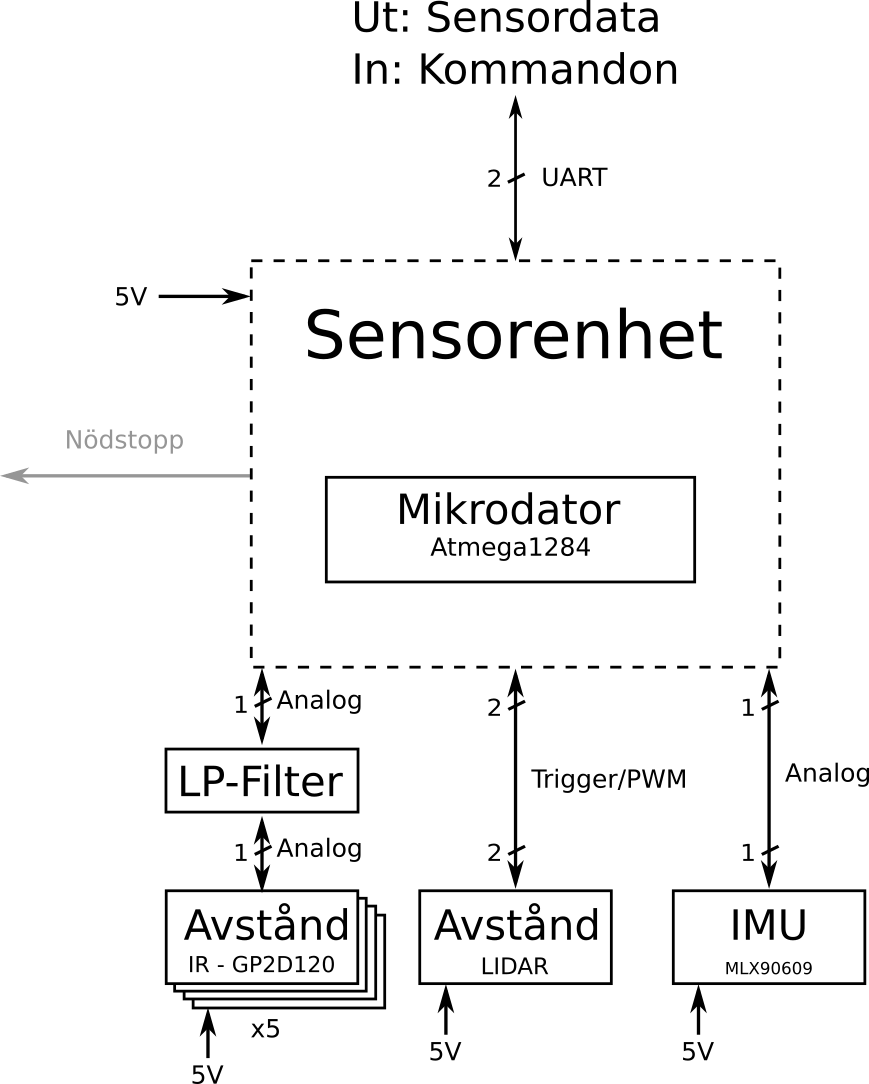
\includegraphics[width=0.6\textwidth]{sensorenhet.png}}
    \caption{Översikt över sensorenheten.}
    \label{fig:unitSensor}
\end{figure}

\noindent \begin{small}
    * Om I\textsuperscript{2}C används krävs även en logic level converter mellan 5V och 3V3 på dessa platser.\\
    ** 5V på Atmega-sidan, 3V3 krävs av sensorn.
\end{small}
\subsection{Hårdvara}

\subsubsection{Processor}
ATmega1284 används som processormodell, då den är kraftfull utan att ta det till överdrift, men även har tillräckligt med avbrottsingångar för att kunna arbeta med LIDARn och samtliga ultraljudssensorer, se \ref{sssec:sonicsensors}.

\subsubsection{Ultraljudssensor} \label{sssec:sonicsensors}
\paragraph{Alternativ 1}
En ultraljudssensor, SRF04, placeras på var och en av robotens fyra sidor och används för navigering och positionsuppskattning. Dessa behöver en utgång och en interrupt-ingång var. Se \ref{ssec:sensorInterface}. Dessa kan användas var 65:e millisekund utan risk för störningar, vilket ger oss möjlighet att läsa av $\sim15$ sensorer per sekund. Troligtvis kan de även användas med mindre eller ingen marginal mellan avläsningarna, men det kräver testning för att avgöras. En annan nackdel är att de fungerar dåligt i vinkel mot en vägg, där de antingen inte ger något värde alls, eller ett ''studsat'' värde. %http://www.robot-electronics.co.uk/htm/sonar_faq.htm

\paragraph{Alternativ 2}
Som alternativ kan IR-sensorer användas. Nackdelen är störningar i den analoga utdatan, som dessutom är ickelinjär, och fungerar på ett kortare intervall än ultraljudssensorer. Fördelen är snabbare avläsningar som troligtvis inte stör varandra. Bredden på mätstrålen är också mindre än med ultraljud.


\subsubsection{LIDAR lite v2} \label{sssec:lidar}
LIDAR är en kraftfull lasersensor som i systemet som helhet används för mätningar som kräver noggranhet. Komponenten kan kommuniceras med via en trigger-pin och PWM-output, alternativt via en I\textsuperscript{2}C-buss. I första hand kommer PWM användas.

Sensorn monteras på toppen av roboten - ovanpå ett roterande servo, som specificeras i större detalj i avsnitt \ref{ssec:servomotor}. Detta för att effektivt kunna mäta avstånd i flera vinklar.

\subsubsection{IMU} \label{sssec:imu}

\paragraph{Alternativ 1}
En enklare modul - exempelvis MLX90609 - används, via en analog ingång. Detta ger oss då endast rotationen kring z-axeln, som kan användas för att beräkna robotens riktning i rummet.

\paragraph{Alternativ 2}
En mer avancerad modul, exempelvis MPU6050, används, via en I\textsuperscript{2}C-buss. Om LIDARn implementerats med I\textsuperscript{2}C delas bussen mellan dessa två. Det ger oss i så fall både riktning och acceleration, för att mer noggrannt kunna beräkna robotens placering.% TODO: MotionMagi, handledare

\subsection{Mjukvara}

Koden ska vara skriven i C, och ska följa standarden specificerad i bilaga \ref{sec:cstandard}.

Programmet ska omvandla sensordata till ett mer läsligt format, och ska kunna skicka det vidare (se \ref{ssec:sensorInterface}).

\subsection{Gränssnitt} \label{ssec:sensorInterface}
Sensorenheten kommer behöva kommunicera med de faktiska sensorerna, samt ha ett sätt att passera vidare utdata. Sensorenheten kan ta emot uppmaningar om att starta en avläsning via samma buss som används för att rapportera mätvärden vidare.

\subsubsection{LIDAR}
LIDAR kommer i första hand använda avläsningstriggers och PWM via en gemensam pin. PWM-signalen kopplas i så fall till ett avbrott för att mäta dess längd, som används för att beräkna avståndet. Som alternativ kan också I\textsuperscript{2}C användas.

\subsubsection{I2C-buss}
Den mer avancerade av IMUerna använder I\textsuperscript{2}C. Även LIDARn kan kommunicera via I\textsuperscript{2}C. Om behov uppstår implementerar vi en I\textsuperscript{2}C-buss. Vi stödjer i så fall inte flera masters, utan behandlar processorn som den enda, med LIDAR:n och gyron som slavar.

\subsubsection{Ultraljudssensorer}
Ultraljudssensorerna (\ref{sssec:sonicsensors}) använder ett liknande gränssnitt som LIDARn, med en trigger-pin och en echo-pin som utgång. Deras utvärde beror på längden av dess höga signal, så för att garantera att vi börjar mäta omedelbart på en hög flank så ska avbrott utnyttjas. Detta uppnås genom att helt enkelt koppla denna signal till en av avbrottsportarna på processorns, för var och en av sensorerna.

\subsubsection{Utvärden/Input}
Hur tas instruktioner emot, samt hur passeras processerade mätvärden vidare?

\paragraph{Alternativ 1}
Implementera en UART-buss som endast går mellan sensorenheten och kommunikationsenheten. Se kapitel \ref{ssec:brainInterface} för mer detaljer om för och nackdelar.

\paragraph{Alternativ 2}
I\textsuperscript{2}C-bussen som eventuellt används för att kommunicera med LIDAR:n och gyron kan utnyttjas, med även processorn som slav. Enheten som tar emot data från/skickar data till sensorenheten får istället ta över rollen som master. Se kapitel \ref{ssec:brainInterface} för mer detaljer om för och nackdelar.

\newpage
\section{Styrenhet} \label{sec:system2}
Styrenheten är ansvarig för robotens lågnivåstyrning. Den är länken mellan alla styrkommandon och motorer. Se figur \ref{fig:unitMotorcontroller} för en övergripande systemskiss för styrenheten.

\begin{figure}[h!]
    \makebox[\textwidth][c]{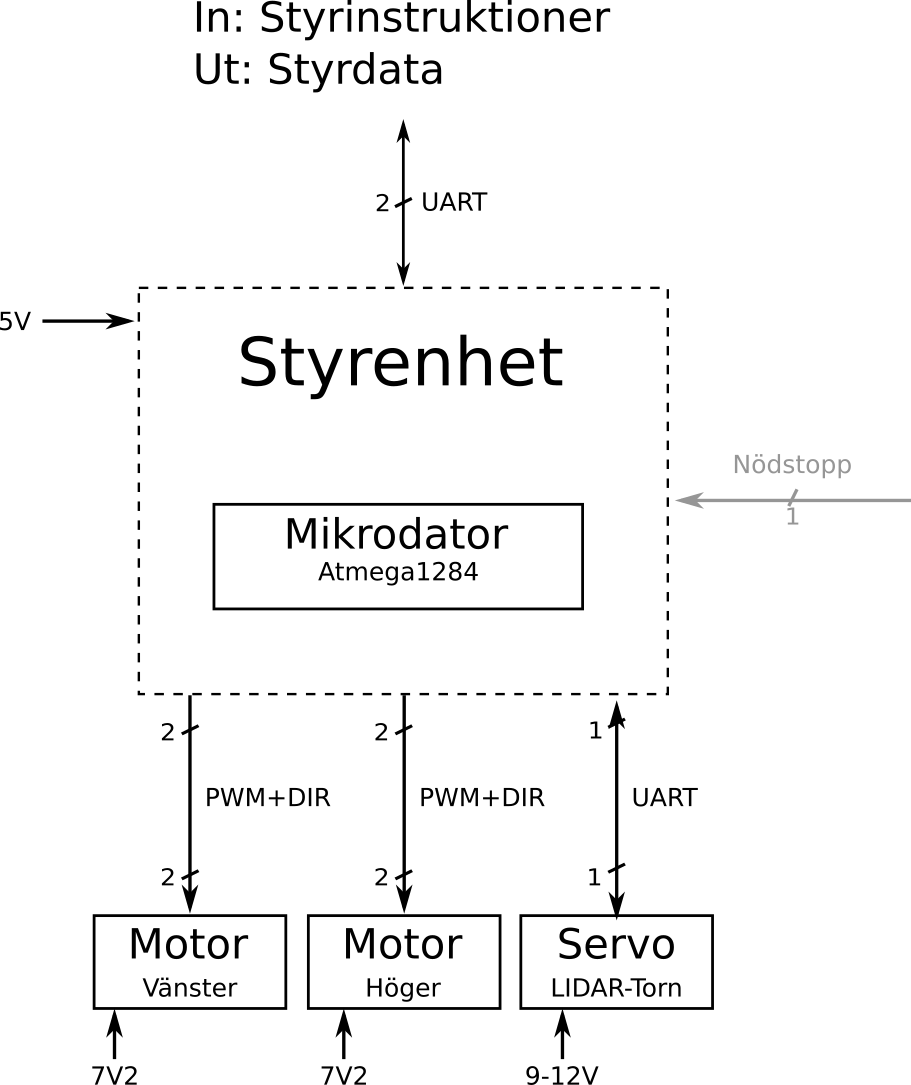
\includegraphics[width=0.6\textwidth]{styrenhet.png}}
    \caption{Översikt över styrenheten.}
    \label{fig:unitMotorcontroller}
\end{figure}

\subsection{Hårdvara}

\subsubsection{Processor}
Vi använder en Atmega1284p-processor för styrmodulen. Processorn kommer totalt att kommunicera med 4 DC-motorer som sitter på chassit (\cite{terminator}) och ett servo. Alla motorerna kommunicerar över PWM.

\subsubsection{Servo/steppermotor} \label{ssec:servomotor}
På toppen av roboten ska en lasersensor (se kapitel \ref{sssec:lidar}) vara monterad, ovanpå en servo som tillåter sensorn att rotera. Servomotorn kommer vara antingen en hobbyservo, som också är våran första prioritet, eller en AX-12(+/A).

\begin{itemize}
%       Om AX-12, skriv något finare än "enligt vissa källor", och faktiskt förklara hur det ligger till.
\item AX-12(+/A) har två rotationslägen: ''vanlig'' och ''wheel''. Det förstnämnda rotationsläget för AX-12:n tillåter oss att göra mycket exakta rotationer, men förhindrar oss från att svänga runt mer än 300 grader. Vi slipper potentiellt felaktiga värden, men kan inte titta rakt bakom oss. Då detta inte är ett stort problem används lämpligen det vanliga läget. Servot använder, enligt vissa källor, 9-12V men klarar sig enligt andra ner emot 7V. Kan alltså eventuellt kräva en step-up-krets från ~7V2 till 9-12V. AX-12:an kommunicerar över half- duplex vilket orsakar endel problem då vi också måste implementera ett sådant protokoll.
%http://support.robotis.com/en/techsupport_eng.htm#product/dynamixel/ax_series/dxl_ax_actuator.ht

\item Hobbyservot kommunicerar över PWM vilket är betydligt enklare att implementera än half-duplex. Svängvidden för hobbyservon brukar vara runt 180 grader.
\end{itemize}

\subsubsection{Hjulmotorer}
Totalt är det fyra motorer som är monterade på chassit. De fyra DC-motorerna styrs parvis (höger sida och vänster sida) med hjälp av en PWM-signal samt en rotationsriktningssignal per motorpar. Sammanlagt används alltså 4 pinnar på processorn för styrning av hjulen.

\subsubsection{Komponentbudget}
Här följer en lista på all hårdvara som detta delsystem kräver.

% TODO add hardware
\begin{HardwareList}
\hardware{Atmega1284p}{Mikroprocessor med 44 pinnar (inklusive 8 A/D-omvandlare).}{1} 
%TODO: Eventuellt LP-filter till AVCC-porten. Finns ej i Anders föreläsning, men i många andra.
\hardware{IQEXO-3}{Occilator för Atmega-klockan, med standardfrekvens 16MHz}{1}
\hardware{Hobbyservo}{Så högt gradtal som möjligt. Dock ej "continuous".}{1}
\hardware{AX-12(+/A)}{Om inte ett Hobbyservo är möjligt.}{1}
\end{HardwareList}

\subsection{Mjukvara}
Koden skrivs i C, och ska följa standarden specificerad i bilaga \ref{sec:cstandard}. Eftersom nödstoppet ska kunna avbryta vad styrmodulen gör när som helst så är det lämpligt att använda avbrott för detta.

\subsubsection{Tillståndsdiagram}
Som vi ser i tillståndsdiagrammet för styrenheten (figur \ref{fig:stateDiagram}) så har vi totalt tre olika tillstånd. Medan styrenheten är i tillståndet \texttt{WAIT} så kommer roboten att stå stilla och invänta en instruktion. Notera att en instruktion kan sättas i alla tillstånd, så om roboten redan har en instruktion inläst då tillståndet sätts till \texttt{WAIT} så kommer roboten börja på denna instruktion omedelbart utan att stanna.

\begin{figure}[h!]
	\makebox[\textwidth][c]{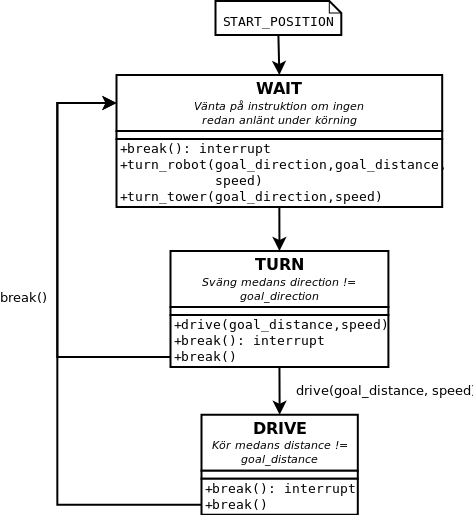
\includegraphics[width=0.5\textwidth]{styrenhet-statediagram.png}}
	\caption{Tillståndsdiagram för styrenheten.}
	\label{fig:stateDiagram}
\end{figure}

\subsubsection{Övergripande programflöde}
I flödesschemat i figur \ref{fig:styrenhetFlowchart} ser vi att det finns funktionalitet som inte avslöjade sig i tillståndsdiagrammet, det vill säga hur vi hanterar de olika instruktionerna \texttt{SCAN} och \texttt{DRIVE}. Om instruktionen är av typen \texttt{SCAN} så kommer aldrig styrenheten att gå in i tillståndet \texttt{TURN} då det inte finns något avstånd att köra. Denna typ av design utesluter givetvis möjligheten att köra och scanna samtidigt. För mer information angående vad de lika instruktionstyperna står för, se kapitel \ref{ssec:controlInterface}. 

\begin{figure}[h!]
\centering
\begin{tikzpicture}[node distance=2cm,scale=0.6, every node/.style={scale=0.6}]
% Styles
\tikzstyle{startstop} = [rounded rectangle, minimum width=3cm, minimum height=1cm,text centered, draw=black, fill=red!30, align=center, inner sep=10pt]
\tikzstyle{io} = [trapezium, trapezium left angle=70, trapezium right angle=110, minimum width=3cm, minimum height=1cm, text centered, draw=black, fill=blue!30, align=center, inner sep=10pt]
\tikzstyle{process} = [rectangle, minimum width=3cm, minimum height=1cm, text centered, draw=black, fill=orange!30, align=center, inner sep=10pt]
\tikzstyle{decision} = [diamond, minimum width=3cm, minimum height=1cm, text centered, draw=black, fill=green!30, align=center, inner sep=10pt, aspect=2]
\tikzstyle{arrow} = [thin,->,>=stealth]

\node (start) [startstop] {Start};
\node (wait_state) [process, below of=start] {\texttt{WAIT\_STATE\_ACTIVATED}};
\node (is_instruction_ready) [decision, right of=wait_state, xshift=6cm] {Any instruction ready \\ to be executed?};
\node (brake) [process, right of=is_instruction_ready, xshift=6cm] {Apply brakes if moving};
\node (turn_state) [process, below of=is_instruction_ready, yshift=-2cm] {\texttt{TURN\_STATE\_ACTIVATED} \\ \\ Turn robot/tower to \\ \texttt{goal\_direction}};
\node (scan_or_drive) [process, below of=turn_state, yshift=-1cm] {Is instruction \texttt{SCAN} or \texttt{DRIVE}?};
\node (drive_state) [process, below of=scan_or_drive, yshift=-0.8cm] {\texttt{DRIVE\_STATE\_ACTIVATED} \\ \\ Drive distance \texttt{goal\_distance}};

\draw [arrow] (start) -- (wait_state);
\draw [arrow] (wait_state) -- (is_instruction_ready);
\draw [arrow] (is_instruction_ready) -- node[auto] {No} (brake);
\draw [arrow] (is_instruction_ready) -- node[auto] {Yes} (turn_state);
\draw [arrow] (turn_state) -- (scan_or_drive);
\draw [arrow] (scan_or_drive) -- node[auto] {\texttt{DRIVE}} (drive_state);
\draw [arrow] (scan_or_drive) -| node[anchor=south, xshift=4cm] {\texttt{SCAN}} (wait_state);
\draw [arrow] (drive_state) -| (wait_state);

\coordinate[above of=is_instruction_ready, yshift=1cm] (d0);
\draw [-] (brake) |- (d0);
\draw [arrow] (d0) -- (is_instruction_ready);


\end{tikzpicture}
	%\makebox[\textwidth][c]{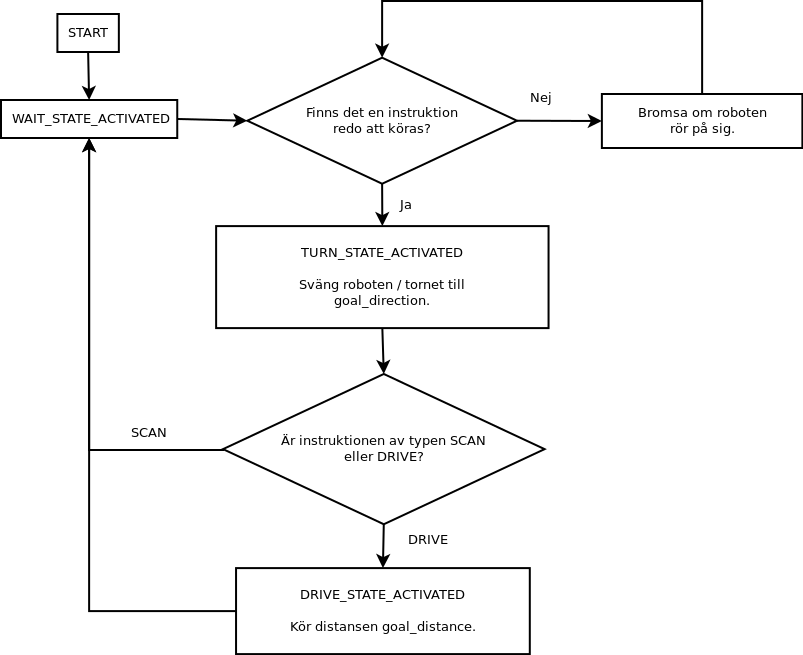
\includegraphics[width=0.9\textwidth]{styrenhet-flowchart.png}}
	\caption{Flödesschema för styrenheten.}
	\label{fig:styrenhetFlowchart}
\end{figure}

\subsubsection{Trådning}
Eftersom att hårdvaran sköter inläsning från en pinne parallellt med det program som körs så behövs mer än en tråd för styrenheten.

\subsection{Reglering}
Eftersom att styrenheten inte har tillgång till data i sensorenheten så blir det kontrollenheten som ansvarar för roboten kör rakt. Styrsignalerna kommer därför innehålla ganska korta sträckor att köra så roboten hinner reglera sin position innan den kör in i en vägg. 

\subsection{Gränssnitt} \label{ssec:controlInterface}

\subsubsection{Styrsignaler samt styrdata}
Vi implementerar en UART-buss som går mellan styrenheten och kommunikationsenheten. Se kapitel \ref{ssec:brainInterface} för mer detaljer om för och nackdelar.

Styrdatan ska innehålla information om följande punkter:
\begin{itemize}
	\item Om instruktionen är av typen \texttt{SCAN} eller \texttt{DRIVE}. \texttt{SCAN} styr servot medans \texttt{DRIVE} styr DC motorerna.
	\item Hur många grader roboten/servot ska rotera.
	\item Hur långt roboten ska köra i den givna riktningen. Denna information är endast intressant om instruktionen är av typen \texttt{DRIVE}.
	\item Vilken hastighet de givna motorerna ska köra med.
\end{itemize}

Från styrenheten skickas information om vilka hastigheter motorerna/servot fått när instruktionen utförs.

\clearpage
\section{Kommunikations- och kontrollenhet} \label{sec:system3}

% SAKER SOM VI INTE GJORT SOM FINNS PÅ CHECKLISTAN:
% Ett kopplingsschema eller väl detaljerat blockschema med namn på signaler och bussar. 
% Vilka avbrott ska användas och vad ska avbrottsrutinerna utföra?

Kommunikations- och kontrollenheten agerar som en central hjärna i systemet. Den tar emot data från de andra delsystemen, och gör val som bidrar till att systemets funktionalitet som helhet uppfylls.

Inga andra delsystem kommunicerar direkt med varandra (förutom ett prio-2-undantag mellan sensorenheten och styrenheten, se kapitel TODO), utan endast med kommunikations- och kontrollenheten. Se figur \ref{fig:unitBrain} för en övergripande skiss.
\begin{figure}[h!]
    \makebox[\textwidth][c]{
\includegraphics[width=1\textwidth]{brain.png}}
    \caption{Översikt över kommunikations- och kontrollenheten.  }
    \label{fig:unitBrain}
\end{figure}

\subsection{Hårdvara}

\subsubsection{Datormodell}
Raspberry pi 3 används, med inbyggd blåtandsmodul. Denna lilla dator är relativt kraftig, och bör därmed inte ha problem med att hålla sitt program gående i rimlig takt. Antalet portar räcker också till: två USB-utgångar behövs för USB-UARTen och två pinnar behövs för brytare och reset-signal (se kapitel \ref{ssec:brainInterface}).

% TODO: kolla om okej mot kravspecen, förhandla med handledare
Då enkortsdatorn kan korrumpera SD-kortet vid brytning av strömmen så kopplas ytterligare en knapp på, som har som funktion att stänga ner mjukvaran. Denna används då lämpligen innan brytaren för strömmen.

För strömförsörjning används en klippt USB-kabel.

\subsubsection{Komponentbudget}
Här följer en lista på all hårdvara som detta delsystem kräver.

\begin{HardwareList}
\hardware{Raspberry Pi 3}{Enkortsdator.}{1}
\hardware{SD-kort}{SD-kort på minst 4GB används som hårddisk.}{1}
\hardware{Klippt USB-kabel}{För strömförsörjning till PI:n.}{1}
\hardware{USB-UART}{Omvandlare för USB till UART}{2}
\hardware{Knapp}{För nedstängning av mjukvara.}{1}
\hardware{Brytare}{Mekaniska brytare för AV/PÅ respektive styrläge.}{2}
\end{HardwareList}

\subsection{Mjukvara}
Koden skrivs i Python 3, och ska följa \cite{pep8}.

\subsubsection{Kommunikation}
Delsystemet är vad som i slutändan kontrollerar de olika delsystemen, och måste därför kunna skicka meddelanden mellan dessa. Mjukvara skrivs för att kunna skicka meddelanden över de olika gränssnitten som den kopplas upp emot (se kapitel \ref{ssec:brainInterface}).

Förutom hårdvarugränssnitt ska den också kunna kommunicera med en extern PC (se kapitel \ref{sec:system4}) med hjälp av blåtandskommunikation, där den kontinuerligt skickar debugdata och kartinformation samt tar emot meddelanden. Dessa meddelanden behandlas i den ordning de köats i pc-mjukvaran och används för att antingen byta läge på roboten, eller för att ge kommandon under manuell styrning. Mjukvaran för blåtandskommunikationen skrivs och ligger som en egen tråd för att utgöra mjukvarukomponenten i kommunikationsmodulen. För en illustration över hur blåtandskommunikationen fungerar, se figur \ref{fig:bluetooth}.

% TODO implementeras UART m.h.a avbrott?
% TODO olika köer för meddelanden från olika ingångar, eller en gemensam? Prioritetskö?
% Vi skulle kunna använda något liknande http://raspi.tv/2013/how-to-use-interrupts-with-python-on-the-raspberry-pi-and-rpi-gpio-part-3
För att hantera meddelanden mellan de interna såväl som de externa modulerna så används köer. Element läggs till i dessa under avbrottsrutiner, men även direkt under mjukvarukörning på olika trådar (Se figur \ref{fig:bluetooth} som exempel). Detta ställer vissa krav på trådsäkerhet och minneskapacitet som inte bör vara något problem att uppnå med kortet.

\begin{figure}[h!]
    \centering
    \begin{tikzpicture}[node distance=2cm,scale=0.6, every node/.style={scale=0.6}]
    \tikzstyle{startstop} = [rounded rectangle, minimum width=3cm, minimum height=1cm,text centered, draw=black, fill=red!30, align=center, inner sep=10pt]
    \tikzstyle{io} = [trapezium, trapezium left angle=70, trapezium right angle=110, minimum width=3cm, minimum height=1cm, text centered, draw=black, fill=blue!30, align=center, inner sep=10pt]
    \tikzstyle{process} = [rectangle, minimum width=3cm, minimum height=1cm, text centered, draw=black, fill=orange!30, align=center, inner sep=10pt]
    \tikzstyle{decision} = [diamond, minimum width=3cm, minimum height=1cm, text centered, draw=black,
    fill=green!30, align=center, inner sep=10pt, aspect=2]
    \tikzstyle{arrow} = [thin,->,>=stealth]
    \tikzstyle{line} = [thin,>=stealth]
    % Nodes
    \node (start) [startstop] {Start};
    \node (initstart) [process, below of=start, yshift=-10pt] {Setup start\\ values};
    \node (connectedquestion) [decision, below of=initstart, yshift=-30pt] {Connected?};
    \node (waitforcom) [io, left of= connectedquestion, xshift=-90pt] {Wait for\\ new connection}; 
    \node (senddata) [process, below of=connectedquestion, yshift=-20pt] {Send data\\ to PC};
    \node (waitforpc) [io, left of=senddata, xshift=-90pt] {Wait for\\ response};
    \node (changemode) [decision, below of=waitforpc, yshift=-20pt] {Change mode?};
    \node (modeswitch) [process, right of=changemode, xshift=90pt] {Switch mode};
    \node (newdata) [decision, below of=changemode, yshift=-40pt] {Commands in\\ response?};
    \node (adddata) [process, below of=newdata, yshift=-30pt] {Add data to\\ input queue};
    % Arrows
    \draw [arrow] (start) -- (initstart);
    \coordinate(dummy2) at ($(initstart) + (0pt,-40pt)$);
    \draw [arrow] (initstart) -- (connectedquestion);
    \draw [arrow] (connectedquestion) -- node[anchor=south] {No}(waitforcom);
    \draw [arrow] (connectedquestion) -- node[auto] {Yes}(senddata);
    \draw [arrow] (senddata) -- (waitforpc);
    \draw [arrow] (waitforpc) -- (changemode);
    \draw [arrow] (changemode) -- node[auto] {No}(newdata);
    \draw [arrow] (changemode) -- node[anchor=south] {Yes}(modeswitch);
    \draw [line] (modeswitch) -- ($(modeswitch) + (83pt,0pt)$); %It works..
    \draw [arrow] (newdata) -- node[auto] {Yes}(adddata);
    \draw [line] (newdata) -- node[auto] {No}($(newdata) + (230pt,0pt)$);
    \coordinate(dummy) at ($(adddata -| newdata) + (230pt,0pt)$);
    \draw [line] (adddata) -- (dummy);
    \draw [line] (dummy) -- (dummy |- connectedquestion);
    \draw [arrow] (dummy |- connectedquestion) -- (connectedquestion);
    \coordinate(test) at (waitforcom |- dummy2);
    \draw [line] (waitforcom |- dummy2) -- (waitforcom);
    \draw [line] (waitforcom |- dummy2) -- (dummy2);
    
    \end{tikzpicture}
    \caption{Programflöde för robotens blåtandskommunikation.}
    \label{fig:bluetooth}
\end{figure}

\subsubsection{Kartritning} \label{sssec:mapping}
Robotens huvuduppdrag är att skanna ett rum och rita en karta över det. Kartan beräknas av kontrollenheten och används internt för bland annat vägletning. Kartan överförs även kontinuerligt till PC:n (se kapitel \ref{sec:system4}) för skärmutritning, så att en användare kan se resultatet.
% TODO Överväg att ha med denna skickning som ett steg i flödesscheman över

\subsubsection{Lägesstyrning}
Roboten konstrueras med två olika lägen: ett manuellt, och ett autonomt. Olika rutiner skrivs för varje, men de delar oundvikligen båda på många funktioner och moduler.

När roboten startar så initieras den med startvärden och hamnar i den huvudloop som ser till att den alltid är i det styrläge som användaren avser, se figur \ref{fig:lageskontroll}.

\begin{figure}[h!]
    \centering
    \begin{tikzpicture}[node distance=2cm,scale=0.6, every node/.style={scale=0.6}]
    \tikzstyle{startstop} = [rounded rectangle, minimum width=3cm, minimum height=1cm,text centered, draw=black, fill=red!30, align=center, inner sep=10pt]
    \tikzstyle{io} = [trapezium, trapezium left angle=70, trapezium right angle=110, minimum width=3cm, minimum height=1cm, text centered, draw=black, fill=blue!30, align=center, inner sep=10pt]
    \tikzstyle{process} = [rectangle, minimum width=3cm, minimum height=1cm, text centered, draw=black, fill=orange!30, align=center, inner sep=10pt]
    \tikzstyle{decision} = [diamond, minimum width=3cm, minimum height=1cm, text centered, draw=black,
     fill=green!30, align=center, inner sep=10pt, aspect=2]
    \tikzstyle{arrow} = [thin,->,>=stealth]
    \tikzstyle{line} = [thin,>=stealth]
    % Nodes
    \node (start) [startstop] {Start};
    \node (initstart) [process, below of=start, yshift=-30pt] {Setup start\\ values};
    \node (exitquestion) [decision, below of=initstart, yshift=-30pt] {Exit?};
    \node (end) [startstop, left of= exitquestion, xshift=-80pt] {End}; %TODO: Behöver vi verkligen det här?
    \node (ismanual) [decision, below of=exitquestion, yshift=-30pt] {Is mode\\ manual?};
    \node (manualmode) [process, right of=ismanual, xshift=100pt] {Run manual mode};
    \node (automode) [process, below of=ismanual, yshift=-30pt] {Run autonomous mode};
    % Arrows
    \draw [arrow] (start) -- (initstart);
    \draw [arrow] (initstart) -- (exitquestion);
    \draw [arrow] (exitquestion) -- node[anchor=south] {Yes}(end);
    \draw [arrow] (exitquestion) -- node[auto] {No}(ismanual);
    \draw [arrow] (ismanual) -- node[anchor=south] {Yes}(manualmode);
    \draw [arrow] (ismanual) -- node[auto] {No}(automode);
    \coordinate(dummy) at ($(manualmode |- automode) + (80pt,0pt)$);
    \draw [line] (automode) -- (dummy);
    \draw [line] (manualmode) -- ($(manualmode) + (80pt,0pt)$);
    \draw [line] (dummy) -- (dummy |- exitquestion); 
    \draw [arrow] (dummy |- exitquestion) -- (exitquestion);
    \end{tikzpicture}
    \caption{Programflöde för robotens huvudloop.}
    \label{fig:lageskontroll}
\end{figure}

\subsubsection{Manuellt läge}
I det manuella läget tar roboten emot kommandon från PC:n via blåtand (se kapitel \ref{sec:system4}) om hur den ska åka, mycket likt en radiostyrd bil. Dessa kommandon motsvarar piltangenterna på ett tangentbord och skickas direkt vidare till styrenheten i form av \texttt{DRIVE}-kommandon (se \ref{sec:system2}). % TODO: Direktlänk.

För testning och felsökning implementeras också följande högnivåkommandon: 

%TODO stämmer dessa?
\begin{table}[h]
\centering
\begin{tabular}{l|l}
Namn & Funktion\\
\hline
\textbf{Fram} & Åk en ruta framåt (40 cm).\\
\textbf{Bak} & Åk en ruta bakåt (40 cm).\\
\textbf{Vänster} & Sväng 90 grader motsols\\
\textbf{Höger} & Sväng 90 grader medsols\\
\textbf{Skanna} & Använd LIDARn (se TODO) för att utföra en skanning\\
\end{tabular}
\caption{En lista på kommandon som ska kunna hanteras i det manuella läget}
\end{table}

\noindent
Kod skrivs för var och en av dessa rutiner, men i ett makroperspektiv blir inte mjukvaran särskilt komplex. Se figur \ref{fig:manual_flowchart} för ett övergripande flödesschema.

\begin{figure}[h!]
\centering
\begin{tikzpicture}[node distance=2cm,scale=0.6, every node/.style={scale=0.6}]
% 
% Skiss:
% Finns meddelande i kön? -Ja-> Utför rutin givet i meddelande
%   |     ʌ     ʌ                       |
%  Nej    |     |                       |
%   |     |     -------------------------
%   V     |
%  Invänta meddelande, dummer!
%
\tikzstyle{startstop} = [rounded rectangle, minimum width=3cm, minimum height=1cm,text centered, draw=black, fill=red!30, align=center, inner sep=10pt]
\tikzstyle{io} = [trapezium, trapezium left angle=70, trapezium right angle=110, minimum width=3cm, minimum height=1cm, text centered, draw=black, fill=blue!30, align=center, inner sep=10pt]
\tikzstyle{process} = [rectangle, minimum width=3cm, minimum height=1cm, text centered, draw=black, fill=orange!30, align=center, inner sep=10pt]
\tikzstyle{decision} = [diamond, minimum width=3cm, minimum height=1cm, text centered, draw=black, fill=green!30, align=center, inner sep=10pt, aspect=2]
\tikzstyle{arrow} = [thin,->,>=stealth]
\tikzstyle{line} = [thin,>=stealth]
% Nodes
\node (start) [startstop] {Start};
\node (com_in_q) [decision, below of=start, yshift=-40pt] {Are there \\queued commands?};
\node (await_com) [io, left of=com_in_q, xshift=-170pt] {Wait for command from PC};
\node (execute) [process, right of=com_in_q, xshift=170pt] {Execute first command in queue};
% Arrows
\draw [arrow] (start) -- (com_in_q);
\draw [arrow] (com_in_q) -- node[anchor=south] {No} (await_com);
\draw [arrow] (com_in_q) -- node[auto] {Yes} (execute);
% Low level drawing cause I can't get this shit working with dummy nodes or fancy arrow paths.
%   - Dummy nodes basically have a small width, meaning we'll have a white square at the turn of the arrow.
%   - Can't figure out how to get arrow paths to turn TWICE.
\draw [line] (await_com) -- ($(await_com) - (0, 100pt)$);
\draw [line] (execute) -- ($(execute) - (0, 100pt)$);
\draw [line] ($(await_com) - (0, 100pt)$) -- ($(execute) - (0, 100pt)$);
\draw [arrow] ($(com_in_q) - (0, 100pt)$) -- (com_in_q);
\end{tikzpicture}
\caption{Typiskt programflöde i det manuella läget. Notera att kön även fylls upp av en separat tråd.}
\label{fig:manual_flowchart}
\end{figure}

\subsubsection{Autonomt läge}
Roboten behöver kontinuerligt ta reda på, leta sig till, och skanna outforskade delar av rummet i det autonoma läget. En algoritm för att hitta ett lämpligt outforskat ställe, en för att hitta en väg dit, och en som skickar lämpliga kommandon till styrenheten (se kapitel \ref{sec:system2}) skrivs. Se figur \ref{fig:auto_flowchart} för ett lämpligt programflöde.

\begin{figure}[h!]
\centering
\begin{tikzpicture}[node distance=2cm,scale=0.6, every node/.style={scale=0.6}]
%
% Skiss:
% Är rummet klarskannat? -Ja-> vägleta till startplats -> klar
%   |        ʌ
%  Nej       |
%   |        ----------------------------------------------------
%   V                                                           |
%  Hitta lämplig rand till outforskat område -> vägleta dit -> skanna
%
% Styles
\tikzstyle{startstop} = [rounded rectangle, minimum width=3cm, minimum height=1cm,text centered, draw=black, fill=red!30, align=center, inner sep=10pt]
\tikzstyle{io} = [trapezium, trapezium left angle=70, trapezium right angle=110, minimum width=3cm, minimum height=1cm, text centered, draw=black, fill=blue!30, align=center, inner sep=10pt]
\tikzstyle{process} = [rectangle, minimum width=3cm, minimum height=1cm, text centered, draw=black, fill=orange!30, align=center, inner sep=10pt]
\tikzstyle{decision} = [diamond, minimum width=3cm, minimum height=1cm, text centered, draw=black, fill=green!30, align=center, inner sep=10pt, aspect=2]
\tikzstyle{arrow} = [thin,->,>=stealth]
% Nodes
\node (start) [startstop] {Start};
\node (complete_map) [decision, below of=start, yshift=-40pt] {Room completely mapped?};
\node (find_border) [process, left of=complete_map, xshift=-200pt] {Find appropriate border to unmapped area};
\node (pathfind) [process, below of=find_border] {Pathfind there};
\node (scan) [process, below of=pathfind] {Scan};
\node (update_map) [process, right of=scan, xshift=200pt] {Update internal map};
\node (pathfind_start) [process, right of=complete_map, xshift=150pt] {Pathfind to start};
\node (done) [startstop, above of=pathfind_start, yshift=40pt] {Done};
% Arrows
\draw [arrow] (start) -- (complete_map);
\draw [arrow] (complete_map) -- node[anchor=south] {No} (find_border);
\draw [arrow] (find_border) -- (pathfind);
\draw [arrow] (pathfind) -- (scan);
\draw [arrow] (scan) -- (update_map);
\draw [arrow] (update_map) -- (complete_map);
\draw [arrow] (complete_map) -- node[auto] {Yes} (pathfind_start);
\draw [arrow] (pathfind_start) -- (done);
\end{tikzpicture}
\caption{Typiskt programflöde i det autonoma läget.}
\label{fig:auto_flowchart}
\end{figure}

\subsection{Gränssnitt} \label{ssec:brainInterface}
Kommunikations- och kontrollenheten använder sig av UART-bussar för datautbyte mellan sensorenhet och styrenhet. Mjukvara för dessa krävs på båda håll. Utbyte av data måste kunna ske åt båda hållen; sensorenheten skickar data på kommando, och styrenheten skickar avlusningsdata.

Utöver detta behövs fungerande blåtandskommunikation. Raspberry PI:ns inbyggda blåtandsmodul används, och vi förväntar oss att PC:n som har användargränssnittet (se kapitel \ref{sec:system4}) även har support för denna typ av kommunikation. I mjukvarulagret används Pythonmodulen \cite{pybluez}.

\newpage
\section{PC} \label{sec:system4}
Detta delsystem kommunicerar med Kommunikations- och kontrollenheten (se kapitel \ref{sec:system3}) för att ta emot diagnostisk data, den upptäckta kartan, samt ge instruktioner vid manuellt läge. Se figur \ref{fig:unitPC} för ett övergripande blockschema över PC-hårdvaran.

\begin{figure}[h!]
    \makebox[\textwidth][c]{
\includegraphics[width=0.6\textwidth]{PC.png}}
    \caption{Översikt över PC-modulen.}
    \label{fig:unitPC}
\end{figure}
\subsection{Hårdvara}
PC-mjukvaran ska vara körbar på en godtycklig PC med Python 3 och blåtandsmodul. Lämpligen med skärm, tangentbord, och datormus för kommunikation med användaren.

\subsubsection{Komponentbudget}
Här följer en lista på all hårdvara som detta delsystem kräver.

\begin{center}
%\begin{HardwareList}
%\hardware{PC}{Bärbar PC med blåtandsmodul}{1}
%\end{HardwareList}
\end{center}

\subsection{Mjukvara}
PC-mjukvaran ansvarar för att kommunicera med roboten över blåtand, låta användaren skicka kommandon till roboten, och visa diagnostik från roboten såväl som kartan. Se figur \ref{fig:gui_flowchart} för ett övergripande flödeschema för PC-mjukvaran. Koden ska vara skriven i Python 3, och ska följa \cite{pep8}.

\begin{figure}[h!]
\centering
\begin{tikzpicture}[node distance=2cm,scale=0.6, every node/.style={scale=0.6}]
% Styles
\tikzstyle{startstop} = [rounded rectangle, minimum width=3cm, minimum height=1cm,text centered, draw=black, fill=red!30, align=center, inner sep=10pt]
\tikzstyle{io} = [trapezium, trapezium left angle=70, trapezium right angle=110, minimum width=3cm, minimum height=1cm, text centered, draw=black, fill=blue!30, align=center, inner sep=10pt]
\tikzstyle{process} = [rectangle, minimum width=3cm, minimum height=1cm, text centered, draw=black, fill=orange!30, align=center, inner sep=10pt]
\tikzstyle{decision} = [diamond, minimum width=3cm, minimum height=1cm, text centered, draw=black, fill=green!30, align=center, inner sep=10pt, aspect=2]
\tikzstyle{arrow} = [thin,->,>=stealth]

% Nodes
\node (start) [startstop] {Start};
\node (bluetooth) [process, below of=start] {Establish Bluetooth \\ connection};
\node (get_gui_event) [io, below of=bluetooth] {Get GUI event};
\node (command_issued) [decision, below of=get_gui_event, yshift=-0.8cm] {GUI command \\ issued?};
\node (should_transmit) [decision, below of=command_issued, yshift=-2cm] {Should \\ command be \\ transmitted?};
\node (perform) [process, right of=should_transmit, xshift=4cm] {Perform command};
\node (is_shutdown) [decision, right of=perform, xshift=3.5cm] {Command is \\ shutdown?};
\node (stop) [startstop, below of=is_shutdown, yshift=-1cm] {Stop};
\node (transmit) [process, below of=should_transmit, yshift=-1cm] {Transmit command};
\node (expecting_reply) [decision, below of=transmit, yshift=-1cm] {Query expecting \\ reply?};
\node (read_reply) [io, below of=expecting_reply, yshift=-1cm] {Read reply};
\node (should_update) [decision, below of=read_reply, yshift=-1cm] {Reply should \\ update GUI?};
\node (issue_event) [process, below of=should_update, yshift=-1cm] {Issue GUI event};

% Arrows
\draw [arrow] (start) -- (bluetooth);
\draw [arrow] (bluetooth) -- (get_gui_event);
\draw [arrow] (get_gui_event) -- (command_issued);
\draw [arrow] (command_issued) -- node[auto] {Yes} (should_transmit);
\draw [arrow] (should_transmit) -- node[auto] {No} (perform);
\draw [arrow] (perform) -- (is_shutdown);
\draw [arrow] (is_shutdown) -- node[auto] {Yes} (stop);
\draw [arrow] (is_shutdown) |- node[anchor=east, xshift=0.8cm, yshift=-5cm] {No} (get_gui_event);
\draw [arrow] (should_transmit) -- node[auto] {Yes} (transmit);
\draw [arrow] (transmit) -- (expecting_reply);
\draw [arrow] (expecting_reply) -- node[auto] {Yes} (read_reply);
\draw [arrow] (read_reply) -- (should_update);
\draw [arrow] (should_update) -- node[auto] {Yes} (issue_event);

% Common decision arrows
\coordinate[left of=get_gui_event, xshift=-3cm] (d1);
\coordinate[left of=issue_event, xshift=-85pt] (d2);
\draw [arrow] (d1) -- (get_gui_event);
\draw [-] (d1) to[below] node[auto] {} (d2);
\draw [-] (issue_event) to[left] node[auto] {} (d2);

\coordinate[left of=should_update, xshift=-85pt] (d3);
\draw [-] (should_update) to[left] node[auto] {No} (d3);

\coordinate[left of=expecting_reply, xshift=-85pt] (d4);
\draw [-] (expecting_reply) to[left] node[auto] {No} (d4);

\coordinate[left of=command_issued, xshift=-85pt] (d5);
\draw [-] (command_issued) to[left] node[auto] {No} (d5);
\end{tikzpicture}
\caption{Typiskt programflöde.}
\label{fig:gui_flowchart}
\end{figure}

% TODO: De andra sektionerna har inte lagt upp det så här med Input/Output-sektioner
%         Kan vara värt att diskutera med resten av gänget eller anpassa sig för ett mer uniformt dokument.

\subsubsection{Input}
PC-mjukvaran tar emot sensordata, styrdata och, kartdata från kommunikationsenheten via blåtand. Den tar också emot instruktioner från mus och tangentbord. 

\subsubsection{Output}
Mjukvaran skickar styrkommandon samt uppmaning om att läsa av sensorerna till roboten i dess manuella läge. Den kan också skicka kommandon om att växla mellan autonomt och manuellt läge, som då går före den fysiska brytaren på roboten.

\subsubsection{GUI}
Informationen som tas emot från roboten presenteras i ett grafiskt gränssnitt. Via det grafiska gränssnittet ska användaren kunna välja kommandon som ska skickas till roboten, se diagnostisk information, växla mellan manuellt och autonomt läge, samt se det hitintills genererade kartan och robotens position i denna. Se figur \ref{fig:gui_mockup} för en mockup.

Det grafiska gränssnittet byggs med grafikbiblioteket \cite{tkinter}.

\begin{figure}[h!]
    \makebox[\textwidth][c]{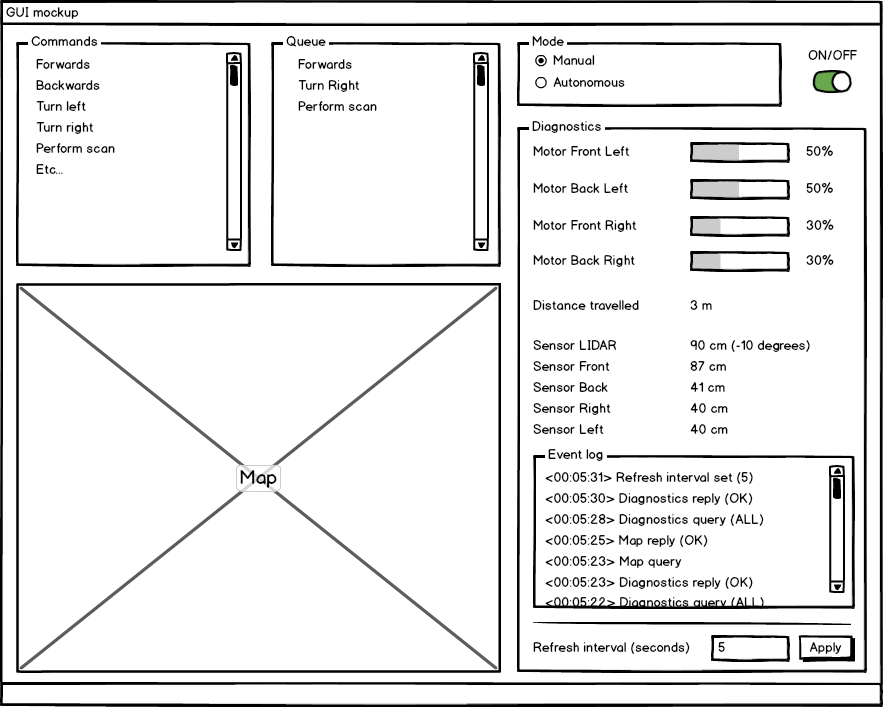
\includegraphics[width=0.8\textwidth]{gui_mockup.png}}
    \caption{Mockup av det grafiska gränssnittet.}
    \label{fig:gui_mockup}
\end{figure}

\subsection{Gränssnitt} \label{ssec:PCInterface}

PC:n kommunicerar med roboten över blåtand. I mjukvarulagret används Pythonmodulen \cite{pybluez}.

\clearpage
\begin{appendices}

\section{Detaljerat blockschema}
% TODO: Sensorenhet-update
\begin{figure}[h!]
    \makebox[\textwidth][c]{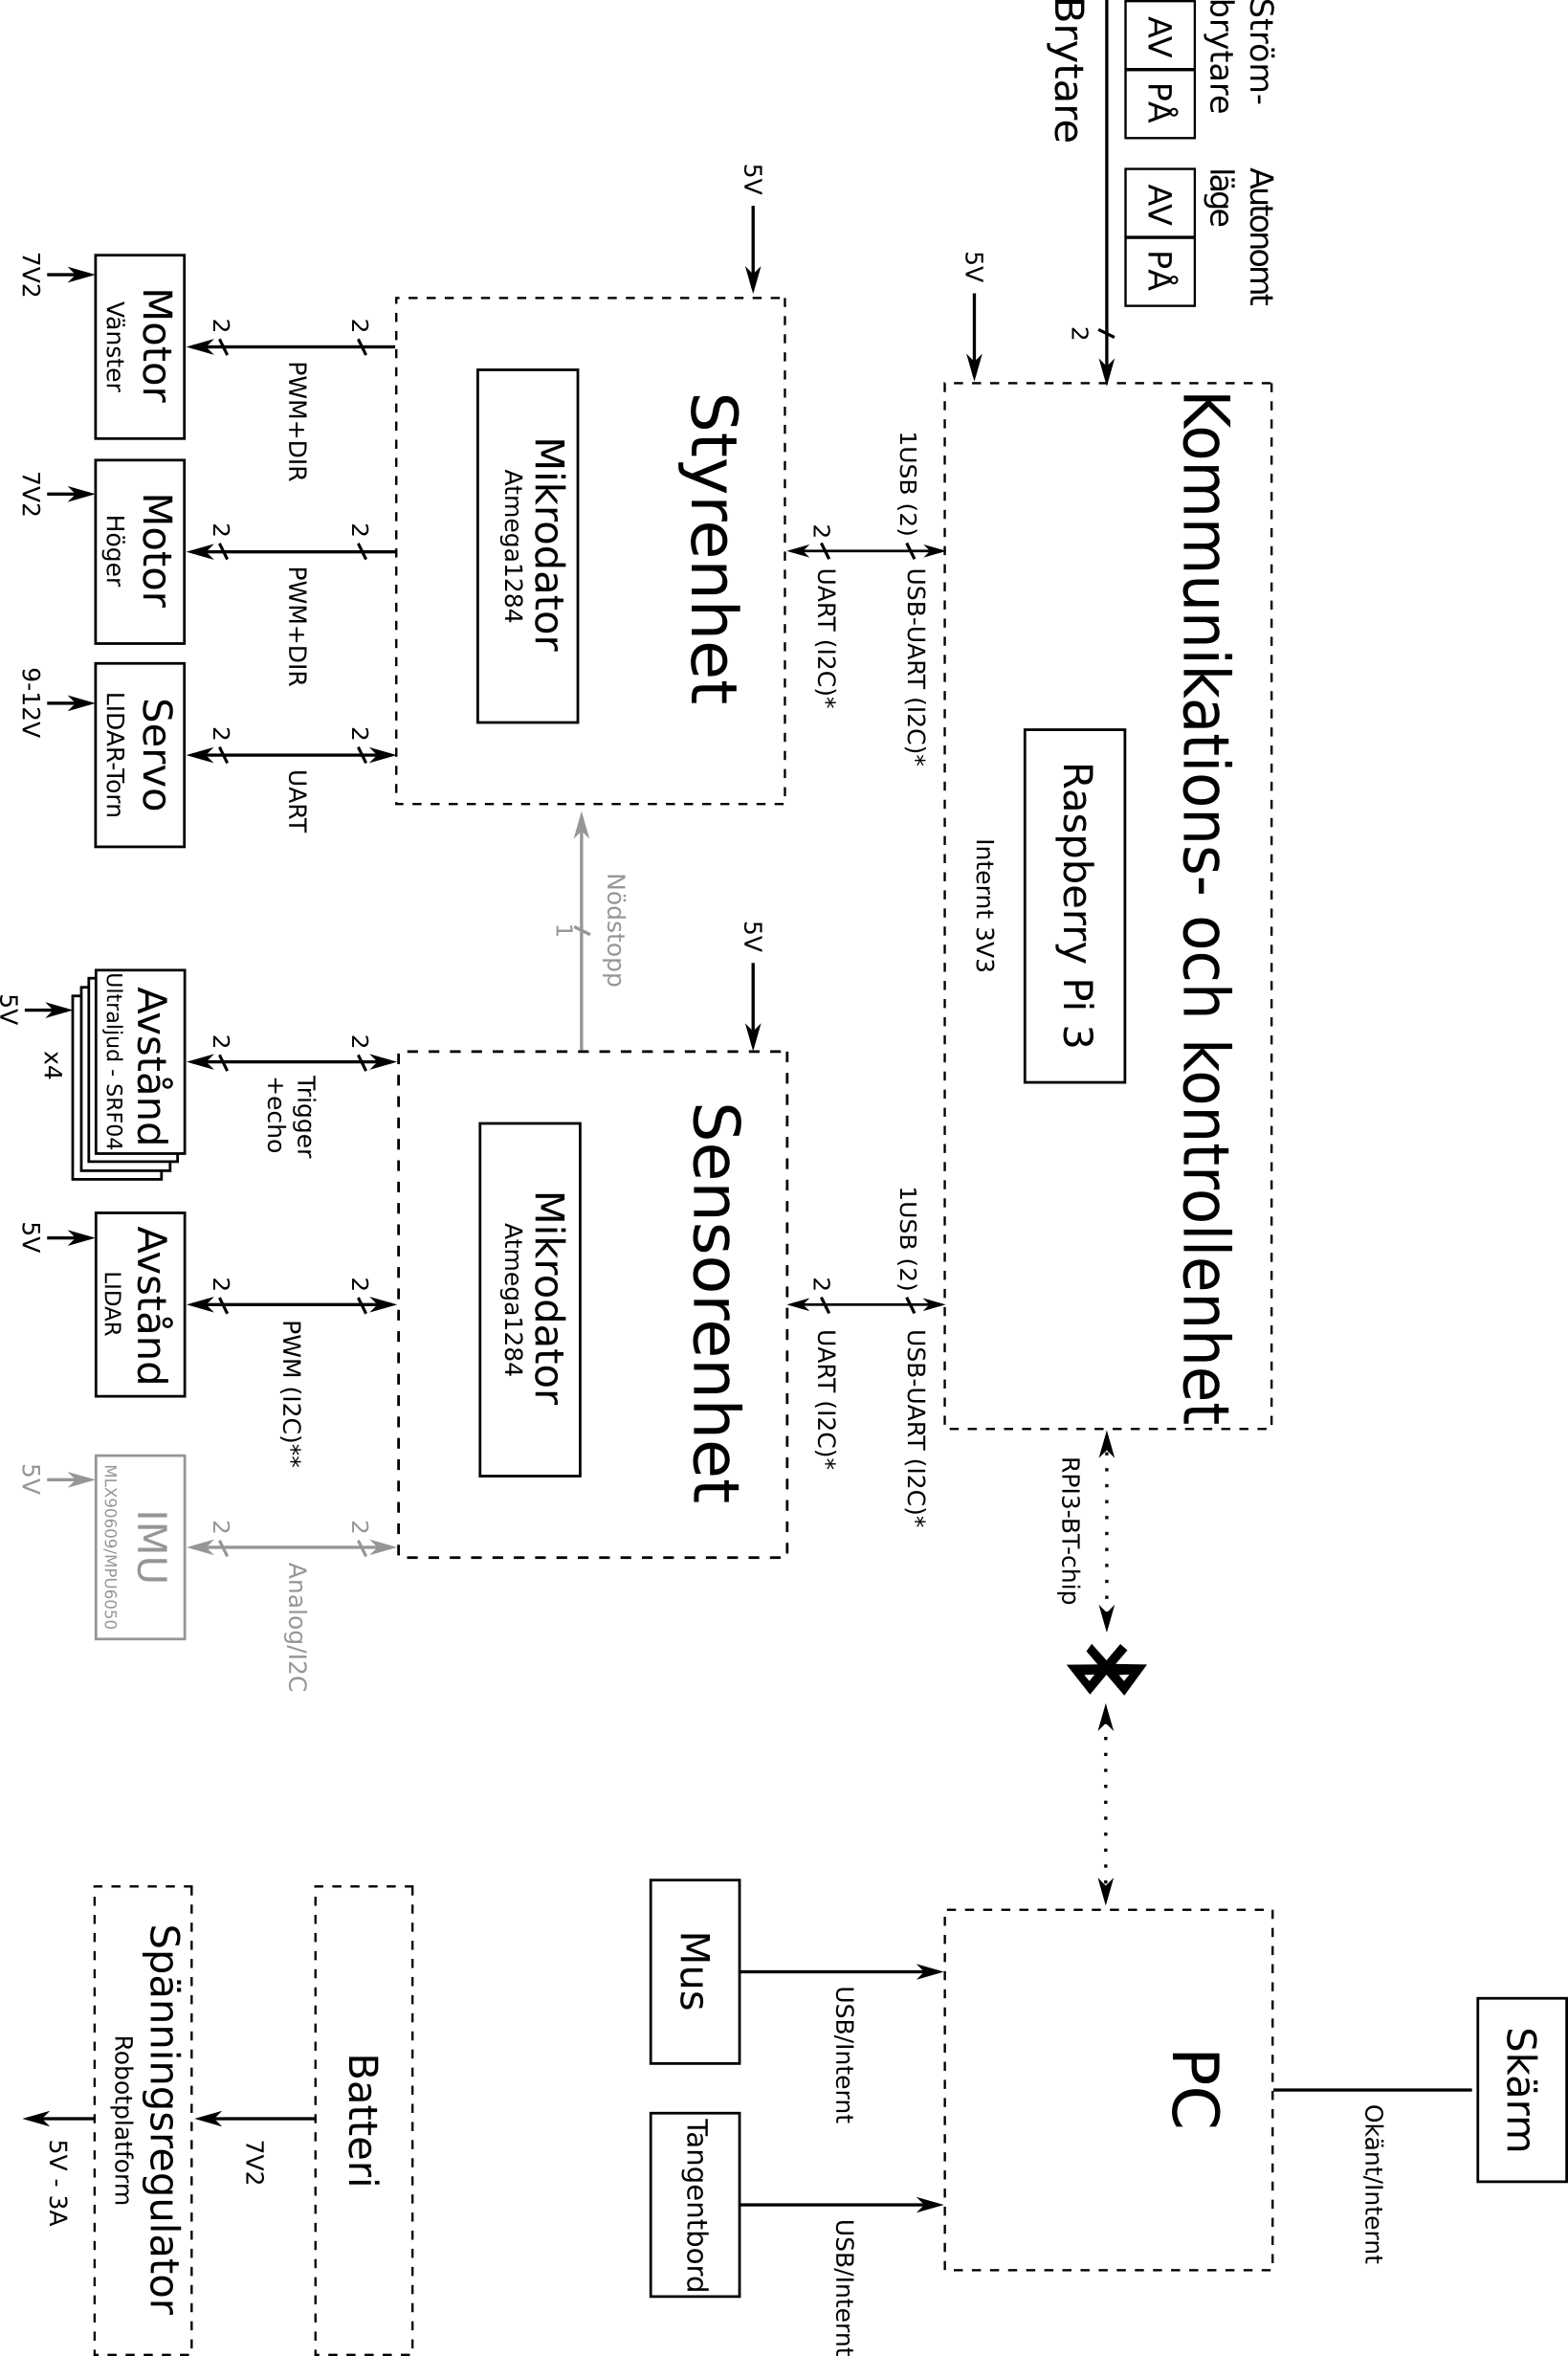
\includegraphics[width=0.9\textwidth]{modules_detail.png}}
    \caption{Detaljerat blockschema över systemet.}
    \label{fig:modulesDetailed}
\end{figure}

\includepdf[scale=0.8,pages=1,angle=180,pagecommand=\section{[Kopplingsschema] Styrenhet}]{schematics/styrenhet/kicad.pdf}

\includepdf[scale=0.8,pages=1,angle=180,pagecommand=\section{[Kopplingsschema] Sensorenhet}]{schematics/sensorenhet/kicad.pdf}

\includepdf[scale=0.8,pages=1,angle=180,pagecommand=\section{[Kopplingsschema] Kontrollenhet}]{schematics/brain/kicad.pdf}

\clearpage
\section{C-standard} \label{sec:cstandard}
Som kodstandard för C används \cite{cstandard} med några smärre tillägg och ändringar:

\begin{itemize}
    \item Indenteringar sker med exakt fyra stycken mellanslag.
    \item Namn på funktioner, typedef, variabler, strukter, unioner, och enums ska vara i lower camel case.
    \item Namn på \#define's, enum-konstanter, och macrofunktioner ska vara i all-caps med ord separerade av underscore.
    \item Typedef:ade namn ska avslutas med "\_t".
    \item Globala namn ska \textit{ej} påbörjas med ett prefix som identiferar vilken modul de tillhör.
    \item Dokumentationskommentarer för funktioner och dylikt ska inledas med "/*" följt av tom rad, med textrader inledda med "{ }* ". Hela kommentaren avslutas med en rad som endast innehåller "{ }*/".
\end{itemize}

\clearpage
\section{Robotplattform}
\label{app:placement}
\begin{figure}[h!]
    \makebox[\textwidth][c]{
\includegraphics[scale=0.6]{layout_topdown_vectorized.png}}
    \caption{Placering av hårdvara på robotchassit.}
    \label{fig:placement}
\end{figure}
\end{appendices}

\clearpage
\addcontentsline{toc}{section}{Referenser} %append references section at this location to TOC
\printbibliography
\end{document}
